% GNUPLOT: LaTeX picture with Postscript
\begingroup
  \makeatletter
  \providecommand\color[2][]{%
    \GenericError{(gnuplot) \space\space\space\@spaces}{%
      Package color not loaded in conjunction with
      terminal option `colourtext'%
    }{See the gnuplot documentation for explanation.%
    }{Either use 'blacktext' in gnuplot or load the package
      color.sty in LaTeX.}%
    \renewcommand\color[2][]{}%
  }%
  \providecommand\includegraphics[2][]{%
    \GenericError{(gnuplot) \space\space\space\@spaces}{%
      Package graphicx or graphics not loaded%
    }{See the gnuplot documentation for explanation.%
    }{The gnuplot epslatex terminal needs graphicx.sty or graphics.sty.}%
    \renewcommand\includegraphics[2][]{}%
  }%
  \providecommand\rotatebox[2]{#2}%
  \@ifundefined{ifGPcolor}{%
    \newif\ifGPcolor
    \GPcolorfalse
  }{}%
  \@ifundefined{ifGPblacktext}{%
    \newif\ifGPblacktext
    \GPblacktexttrue
  }{}%
  % define a \g@addto@macro without @ in the name:
  \let\gplgaddtomacro\g@addto@macro
  % define empty templates for all commands taking text:
  \gdef\gplbacktext{}%
  \gdef\gplfronttext{}%
  \makeatother
  \ifGPblacktext
    % no textcolor at all
    \def\colorrgb#1{}%
    \def\colorgray#1{}%
  \else
    % gray or color?
    \ifGPcolor
      \def\colorrgb#1{\color[rgb]{#1}}%
      \def\colorgray#1{\color[gray]{#1}}%
      \expandafter\def\csname LTw\endcsname{\color{white}}%
      \expandafter\def\csname LTb\endcsname{\color{black}}%
      \expandafter\def\csname LTa\endcsname{\color{black}}%
      \expandafter\def\csname LT0\endcsname{\color[rgb]{1,0,0}}%
      \expandafter\def\csname LT1\endcsname{\color[rgb]{0,1,0}}%
      \expandafter\def\csname LT2\endcsname{\color[rgb]{0,0,1}}%
      \expandafter\def\csname LT3\endcsname{\color[rgb]{1,0,1}}%
      \expandafter\def\csname LT4\endcsname{\color[rgb]{0,1,1}}%
      \expandafter\def\csname LT5\endcsname{\color[rgb]{1,1,0}}%
      \expandafter\def\csname LT6\endcsname{\color[rgb]{0,0,0}}%
      \expandafter\def\csname LT7\endcsname{\color[rgb]{1,0.3,0}}%
      \expandafter\def\csname LT8\endcsname{\color[rgb]{0.5,0.5,0.5}}%
    \else
      % gray
      \def\colorrgb#1{\color{black}}%
      \def\colorgray#1{\color[gray]{#1}}%
      \expandafter\def\csname LTw\endcsname{\color{white}}%
      \expandafter\def\csname LTb\endcsname{\color{black}}%
      \expandafter\def\csname LTa\endcsname{\color{black}}%
      \expandafter\def\csname LT0\endcsname{\color{black}}%
      \expandafter\def\csname LT1\endcsname{\color{black}}%
      \expandafter\def\csname LT2\endcsname{\color{black}}%
      \expandafter\def\csname LT3\endcsname{\color{black}}%
      \expandafter\def\csname LT4\endcsname{\color{black}}%
      \expandafter\def\csname LT5\endcsname{\color{black}}%
      \expandafter\def\csname LT6\endcsname{\color{black}}%
      \expandafter\def\csname LT7\endcsname{\color{black}}%
      \expandafter\def\csname LT8\endcsname{\color{black}}%
    \fi
  \fi
    \setlength{\unitlength}{0.0500bp}%
    \ifx\gptboxheight\undefined%
      \newlength{\gptboxheight}%
      \newlength{\gptboxwidth}%
      \newsavebox{\gptboxtext}%
    \fi%
    \setlength{\fboxrule}{0.5pt}%
    \setlength{\fboxsep}{1pt}%
\begin{picture}(8496.00,3528.00)%
    \gplgaddtomacro\gplbacktext{%
      \csname LTb\endcsname%
      \put(770,902){\makebox(0,0){\strut{}$-1$}}%
      \put(1358,828){\makebox(0,0){\strut{}$0$}}%
      \put(1947,755){\makebox(0,0){\strut{}$1$}}%
      \put(2534,681){\makebox(0,0){\strut{}$2$}}%
      \put(2771,722){\makebox(0,0){\strut{}$-1$}}%
      \put(3167,871){\makebox(0,0){\strut{}$0$}}%
      \put(3564,1021){\makebox(0,0){\strut{}$1$}}%
      \put(3960,1170){\makebox(0,0){\strut{}$2$}}%
      \put(459,1069){\makebox(0,0)[r]{\strut{}$-1$}}%
      \put(459,1475){\makebox(0,0)[r]{\strut{}$0$}}%
      \put(459,1880){\makebox(0,0)[r]{\strut{}$1$}}%
      \put(459,2286){\makebox(0,0)[r]{\strut{}$2$}}%
      \put(-75,1780){\makebox(0,0){\strut{}z}}%
    }%
    \gplgaddtomacro\gplfronttext{%
      \csname LTb\endcsname%
      \put(1318,609){\makebox(0,0){\strut{}x}}%
      \put(3753,751){\makebox(0,0){\strut{}y}}%
      \put(-75,1780){\makebox(0,0){\strut{}z}}%
    }%
    \gplgaddtomacro\gplbacktext{%
      \csname LTb\endcsname%
      \put(4540,831){\makebox(0,0)[r]{\strut{}$-6$}}%
      \put(4540,1306){\makebox(0,0)[r]{\strut{}$-4$}}%
      \put(4540,1782){\makebox(0,0)[r]{\strut{}$-2$}}%
      \put(4540,2258){\makebox(0,0)[r]{\strut{}$0$}}%
      \put(4540,2733){\makebox(0,0)[r]{\strut{}$2$}}%
      \put(4540,3209){\makebox(0,0)[r]{\strut{}$4$}}%
      \put(4672,373){\makebox(0,0){\strut{}$0$}}%
      \put(5420,373){\makebox(0,0){\strut{}$2$}}%
      \put(6167,373){\makebox(0,0){\strut{}$4$}}%
      \put(6915,373){\makebox(0,0){\strut{}$6$}}%
      \put(7662,373){\makebox(0,0){\strut{}$8$}}%
      \put(8410,373){\makebox(0,0){\strut{}$10$}}%
    }%
    \gplgaddtomacro\gplfronttext{%
      \csname LTb\endcsname%
      \put(4232,1901){\rotatebox{-270}{\makebox(0,0){\strut{}energy}}}%
      \put(6541,208){\makebox(0,0){\strut{}time t}}%
      \csname LTb\endcsname%
      \put(7480,2279){\makebox(0,0)[r]{\strut{}Kinetic energy}}%
      \csname LTb\endcsname%
      \put(7480,2059){\makebox(0,0)[r]{\strut{}Potential energy}}%
      \csname LTb\endcsname%
      \put(7480,1839){\makebox(0,0)[r]{\strut{}Total energy}}%
    }%
    \gplbacktext
    \put(0,0){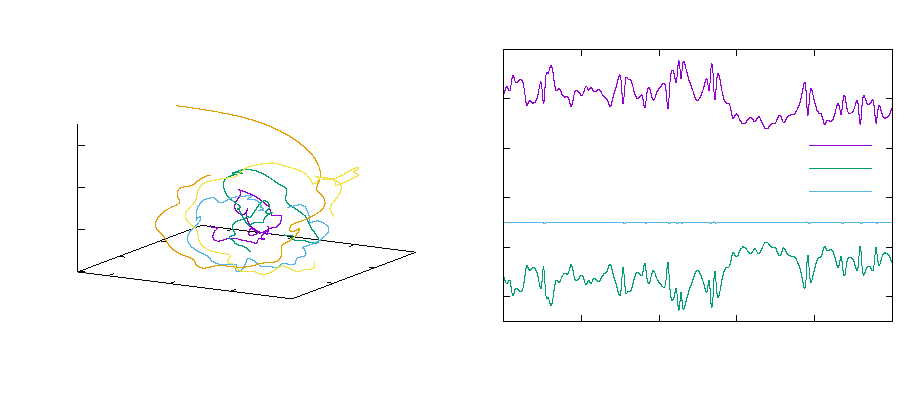
\includegraphics{MDSLP3N5}}%
    \gplfronttext
  \end{picture}%
\endgroup
